\chapter{Introduzione, Architettura e Infrastruttura}

\section{Evoluzione: Dalle Sale Server alle AI Factories}
\begin{figure}[H]
    \centering
    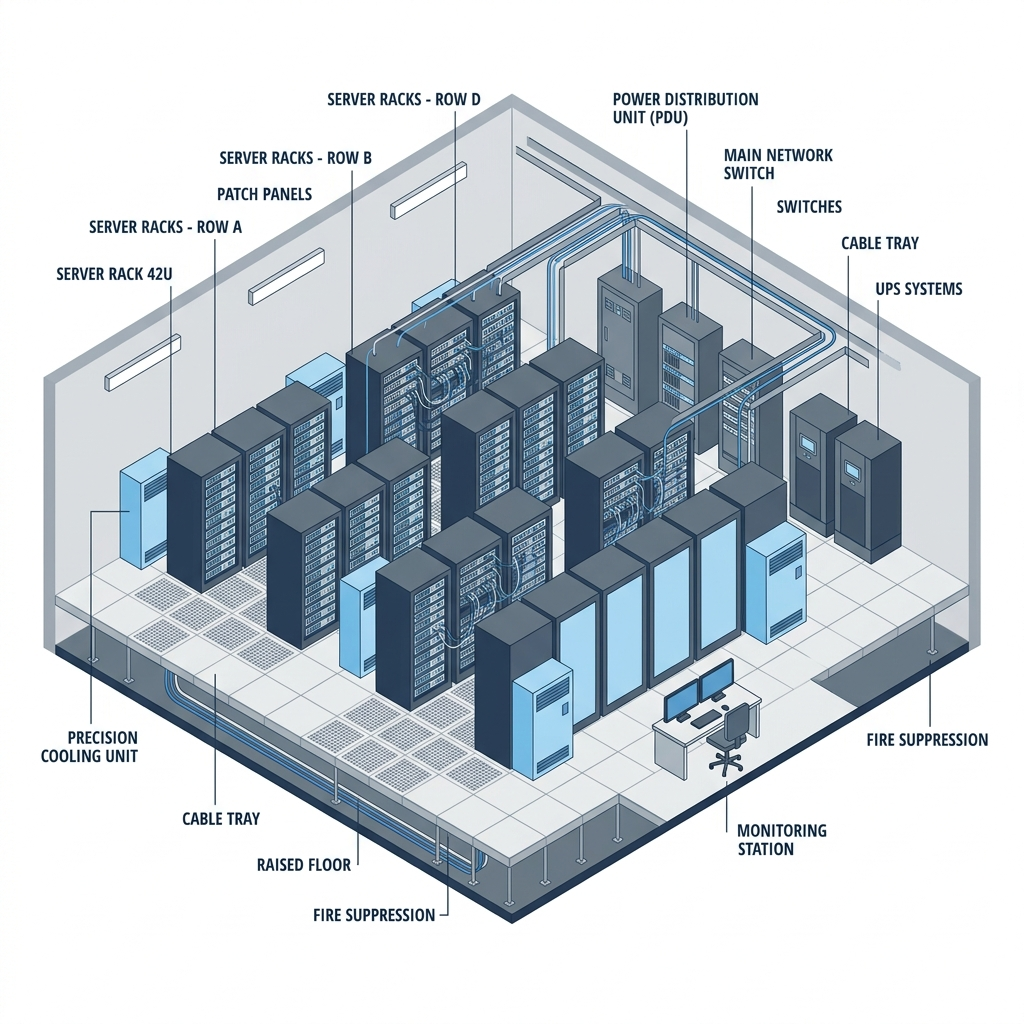
\includegraphics[width=0.8\textwidth]{images/datacenter_isometric.png}
    \caption{Illustrazione isometrica di un moderno datacenter ad alta densità.}
\end{figure}
\subsection{Dai Mainframe alla Bolla delle Dot-Com}
Storicamente, il calcolo centralizzato nasce negli anni '60 e '70 con i \textbf{Mainframe} (es. sistemi IBM): giganteschi armadi chiusi in stanze asettiche ("glass house") a cui gli utenti accedevano tramite terminali stupidi (green screen). In questa fase, il sistema era un blocco monolitico proprietario e altamente centralizzato.
Negli anni '80 e '90 si passa al modello \textbf{Client-Server}, con i server x86 (architettura aperta) distribuiti in semplici "sale server" aziendali, spesso ex ripostigli riadattati con un condizionatore commerciale e nessuna vera progettazione ingegneristica.
Alla fine degli anni '90, l'esplosione di Internet porta alla \textbf{bolla delle Dot-Com}: la necessità di scalare globalmente spinge le aziende ad affittare spazio (Colocation) in giganteschi edifici specializzati gestiti da telco e provider, per garantire l'accessibilità H24. Da qui nasce il vero e proprio concetto moderno di Datacenter.

\subsection{L'Era dell'Intelligenza Artificiale e la Top500}
Oggi si tratta di un'infrastruttura critica a livello nazionale, che richiede investimenti dell'ordine di centinaia di milioni, se non miliardi, di euro. 
L'esplosione dell'intelligenza artificiale (IA) ha portato all'era delle \textbf{AI Factories}: complessi industriali in grado di assorbire fino a 1-2 Gigawatt, l'equivalente di un'intera città.
La potenza di questi cluster è costantemente tracciata da due classifiche mondiali semestrali (nate nel 1993):
\begin{itemize}
    \item \textbf{Top500:} Misura le prestazioni assolute (benchmark di algebra lineare in PetaFLOPS).
    \item \textbf{Green500:} Misura l'efficienza energetica (GigaFLOPS per Watt), evidenziando il profondo \textbf{impatto ambientale} di queste strutture.
\end{itemize}

L'IA ha radicalmente alterato i paradigmi del passato: mentre nel Cloud computing tradizionale si sfrutta la virtualizzazione per massimizzare l'uso dell'hardware (normalmente inattivo per il 90\% del tempo), l'IA è il primo \textit{workload} che \textbf{satura integralmente l'hardware fisico}. Questo rende la virtualizzazione inutile nello stack AI e impone l'utilizzo di architetture hardware distribuite su decine di migliaia di GPU interconnesse.

\section{Fondamenti e Vincoli Fisici}
La costruzione di un datacenter moderno si scontra con limiti ingegneristici definiti \textbf{Hard Thresholds}: soglie fisiche oltre le quali non è possibile semplicemente "scalare" (ingrandire) una tecnologia, ma diventa necessario un ripensamento radicale.

\begin{warningbox}[Attenzione: Scale Up vs Scale Out]
\begin{itemize}
    \item \textbf{Scale Out:} aggiungere nuovi nodi o server per distribuire il carico.
    \item \textbf{Scale Up:} aumentare la capacità del singolo nodo (o, nel caso elettrico, del singolo cavo o edificio).
\end{itemize}
L'infrastruttura elettrica di un intero datacenter è costretta a operare in logica \textbf{Scale Up}: all'aumentare del consumo occorrono cavi in rame via via più spessi e costosi.
\end{warningbox}

\subsection{Pavimento Flottante}
\begin{figure}[H]
    \centering
    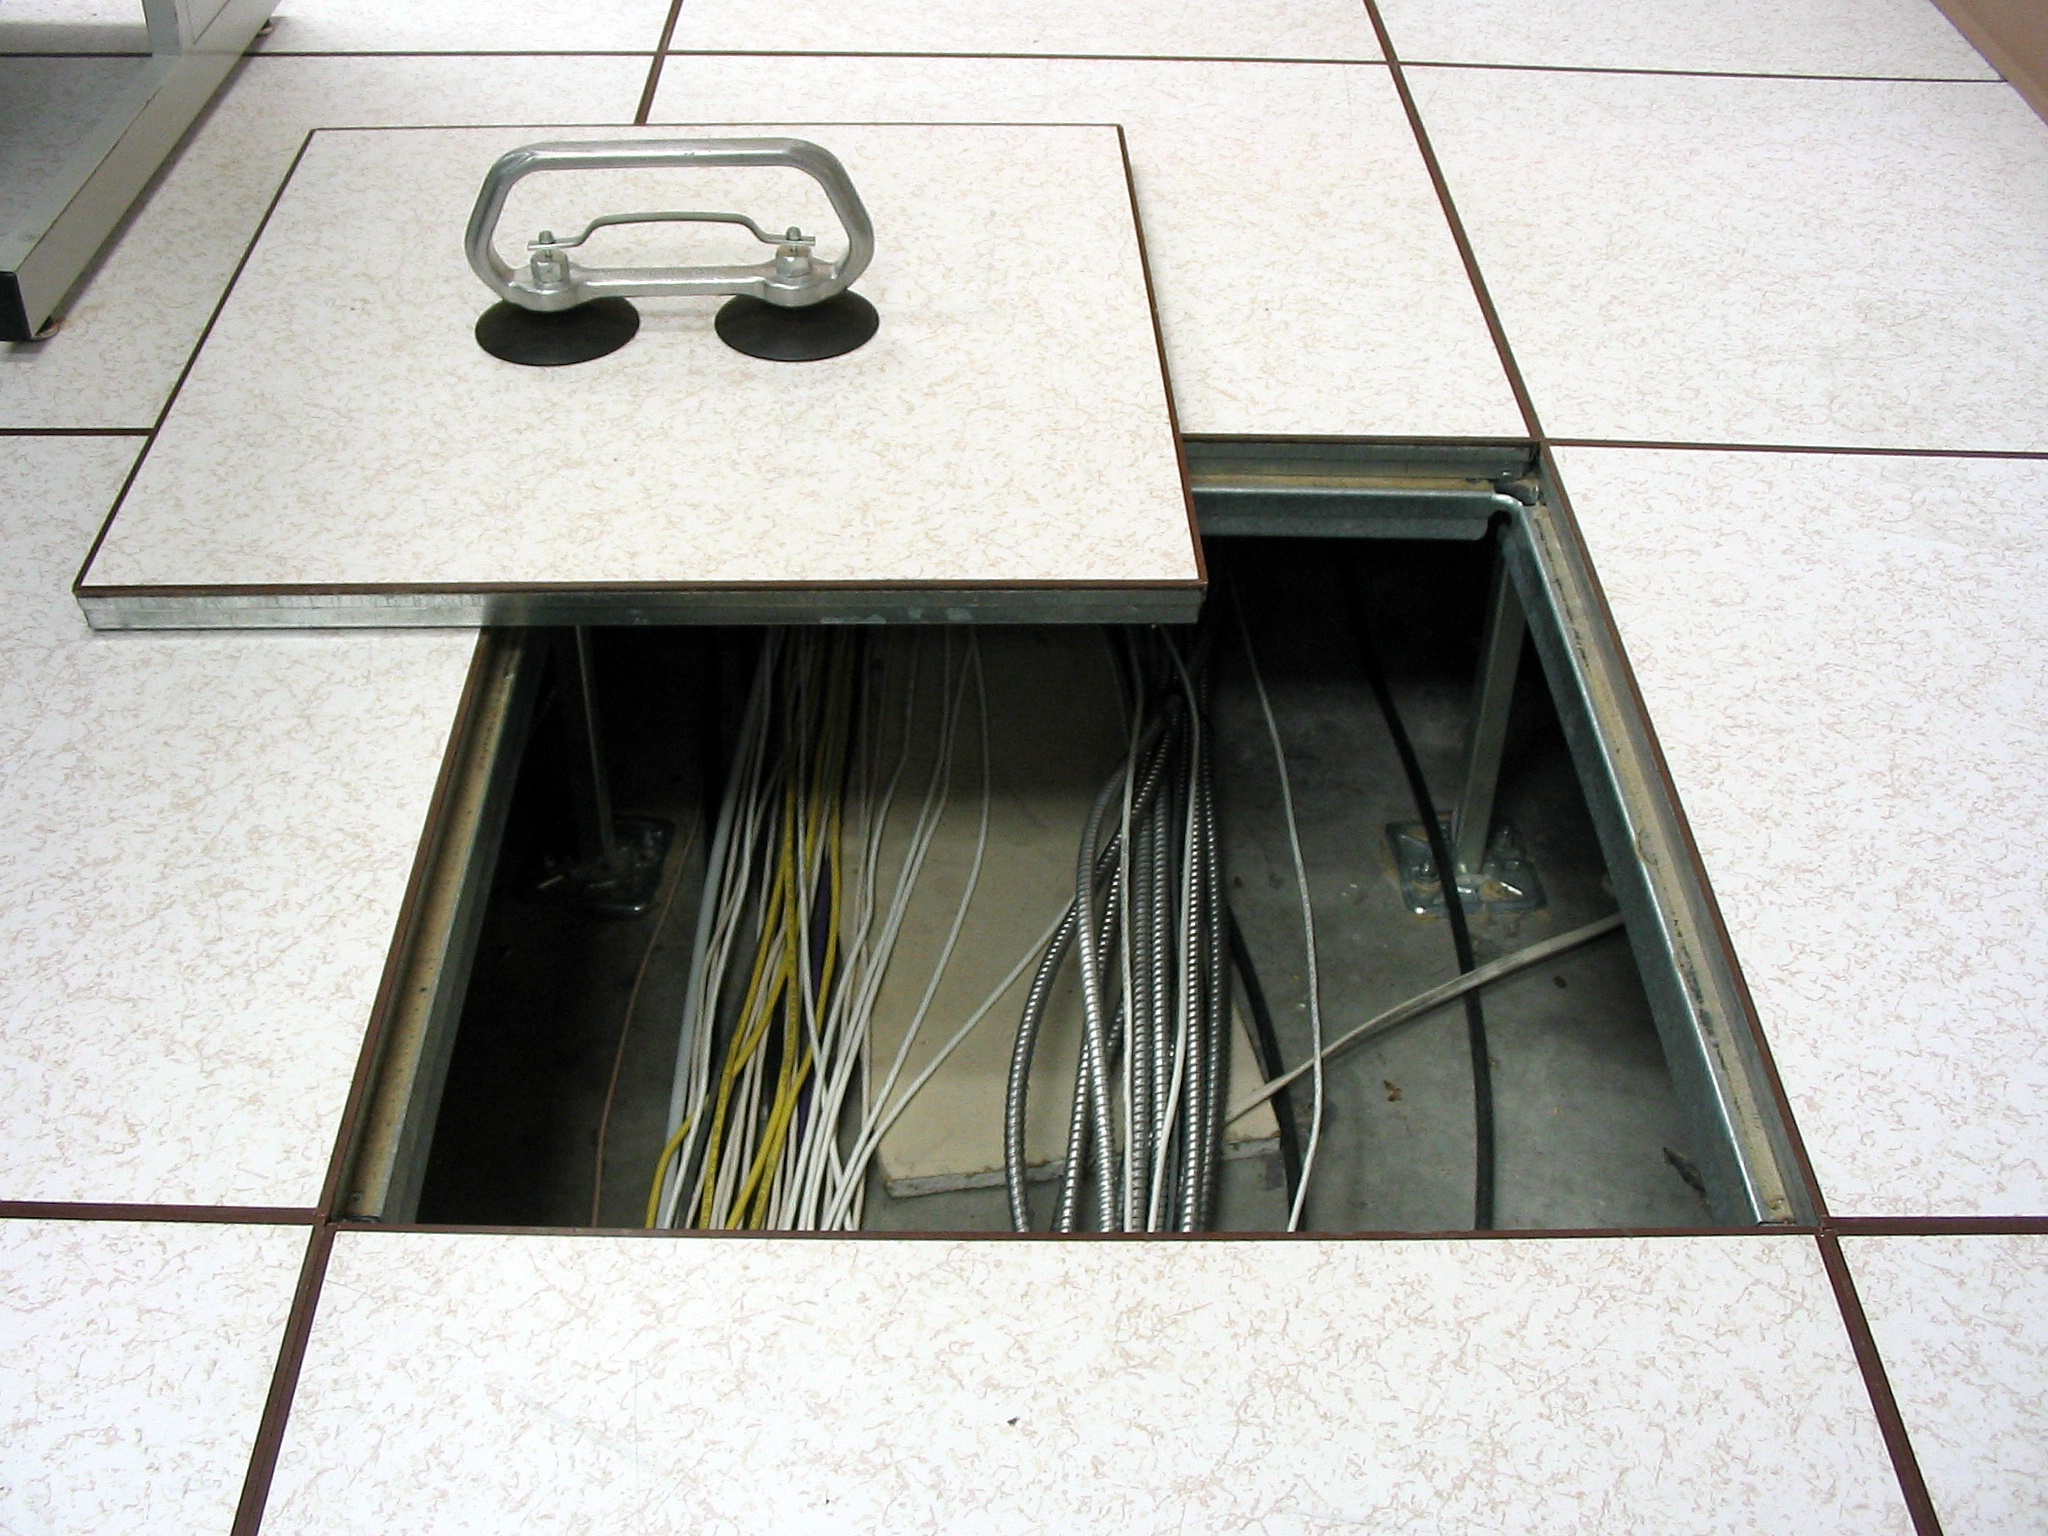
\includegraphics[width=0.7\textwidth]{images/raised_floor.jpg}
    \caption{Sollevamento di una piastrella dal pavimento flottante in un data center (Wikimedia Commons).}
\end{figure}
Una delle eredità ingegneristiche più diffuse è il \textbf{Floating Floor} (pavimento flottante). Costituito da pannelli sollevati su piedistalli metallici, nei moderni DC può reggere fino a 1.5 tonnellate per metro quadrato.
I due grandi vantaggi sono:
\begin{enumerate}
    \item \textbf{Gestione cavi:} passaggio ordinato dell'infrastruttura di cablaggio e tubazioni idrauliche.
    \item \textbf{Plenum per l'aria:} creazione di un condotto pressurizzato sotto il pavimento per distribuire l'aria fredda dal sistema di raffreddamento verso le griglie posizionate di fronte ai rack.
\end{enumerate}

\section{Raffreddamento e Gestione Termica}
A causa dell'estrema densità di calore, dovuta all'elevato \textbf{TDP (Thermal Design Power)} dei nuovi processori (che raggiungono il Kilowatt per singola GPU), il controllo termico è diventato l'aspetto più critico del design. 
La temperatura estrema può fondere i componenti in silicio; l'interruzione del sistema di raffreddamento, unita al tentativo delle ventole dei server di spingere aria, causa aumenti termici esponenziali che possono danneggiare l'intera stanza in pochissimi minuti.

\subsection{L'Architettura ad Aria: Sistemi CRAC e Flussi}
\begin{figure}[H]
    \centering
    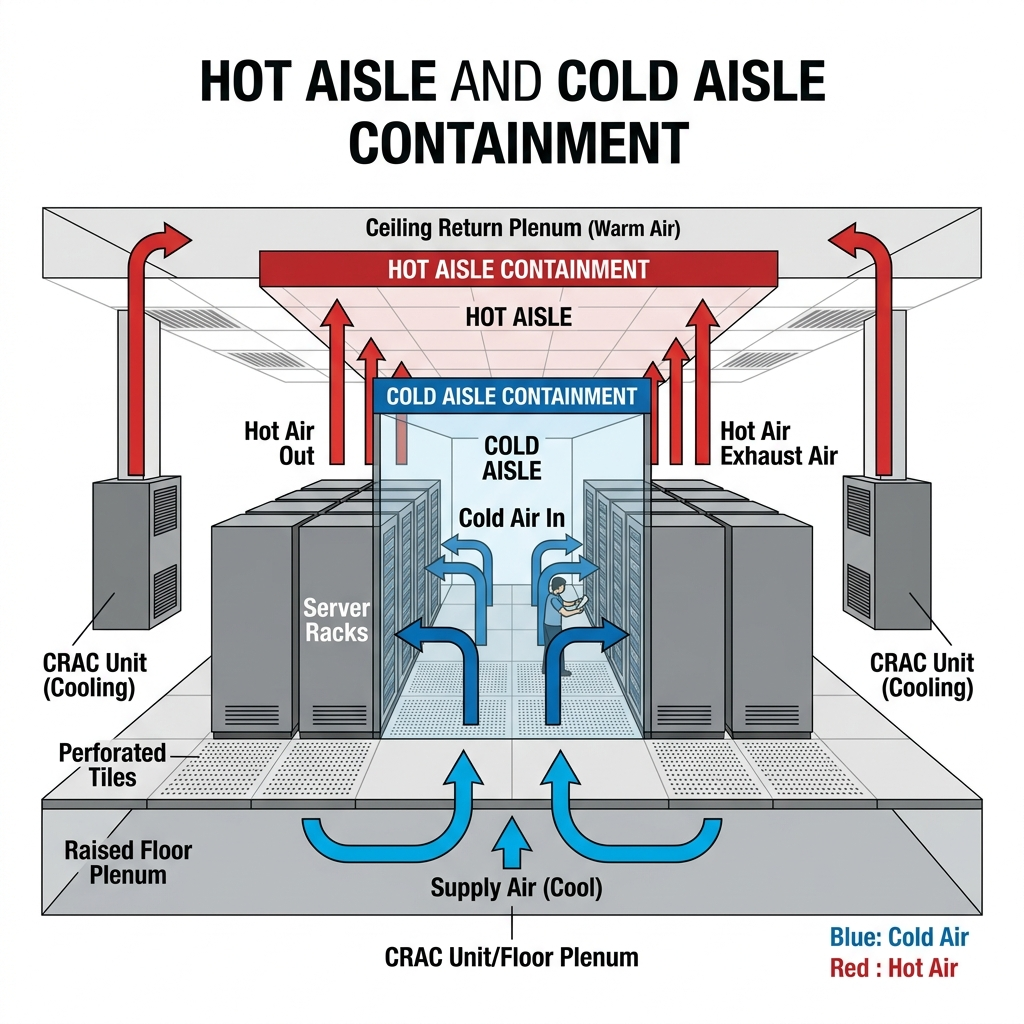
\includegraphics[width=0.8\textwidth]{images/aisle_containment.png}
    \caption{Schema del flusso d'aria: contenimento del corridoio freddo (Cold Aisle Containment) e corridoio caldo.}
\end{figure}
I sistemi \textbf{CRAC (Computer Room Air Conditioning)} si basano sul pavimento flottante e sul principio della rigorosa separazione tra \textit{Cold Aisle} (corridoio freddo) e \textit{Hot Aisle} (corridoio caldo). 
Il flusso dell'aria segue un percorso preciso: le unità CRAC immettono aria ghiacciata pressurizzata nel \textit{plenum} (lo spazio sotto il pavimento flottante). L'aria fuoriesce dalle grate forate esattamente di fronte ai rack (Cold Aisle). Le ventole dei server risucchiano l'aria frontalmente, raffreddano i dissipatori interni, ed espellono l'aria rovente dal retro nel corridoio caldo (Hot Aisle), dove sale verso il soffitto per tornare ai CRAC ed essere raffreddata nuovamente tramite scambiatori di calore ad acqua (Chiller).

\begin{tipbox}[Regola Aurea]
Mai mescolare l'aria calda e l'aria fredda. Se i flussi si mescolano, l'efficienza crolla e le CPU rischiano il \textit{thermal throttling}. Per questo si usano porte a vetri e tettucci chiusi per creare sistemi di \textbf{contenimento fisico} dei corridoi.
\end{tipbox}

Tuttavia, l'aria è un pessimo conduttore termico. Per carichi elevati (Rack oltre i 15-20 kW, per non parlare dei moderni rack AI da 200 kW), i sistemi CRAC ad aria sono insufficienti.

\subsection{Liquid Cooling}
Il raffreddamento a liquido è oggi uno standard di fatto per l'high performance computing (HPC):
\begin{itemize}
    \item \textbf{Direct-to-Chip:} placche di rame raffreddate ad acqua poste direttamente a contatto con CPU, GPU e RAM. Rimuove la necessità di ventole ad alta velocità.
    \item \textbf{Waterless Cooling:} utilizzo di fluidi dielettrici (es. glicole) in tubazioni. In caso di sversamento, non causano cortocircuiti.
    \item \textbf{Immersion Cooling:} immersione completa della scheda madre in olio minerale. Elimina ogni punto di calore localizzato (hot-spot), ma rende la manutenzione complessa e costosa.
\end{itemize}

\section{L'Efficienza Energetica (PUE)}
L'efficienza di un datacenter si misura con un valore adimensionale standard, il \textbf{PUE (Power Usage Effectiveness)}:
\[
PUE = \frac{\text{Total Facility Power}}{\text{IT Equipment Power}}
\]
Più il PUE si avvicina a 1, maggiore è l'efficienza (significa che non si sta sprecando energia per raffreddare). I migliori data center odierni hanno un PUE annuo attorno a 1.15 - 1.20.

\section{Sicurezza e Continuità}
La progettazione logica segue la cosiddetta \textbf{CIA Triad}:
\begin{itemize}
    \item \textbf{C}onfidentiality (Riservatezza)
    \item \textbf{I}ntegrity (Integrità)
    \item \textbf{A}vailability (Disponibilità)
\end{itemize}

L'approvvigionamento elettrico è vitale. La distribuzione avviene seguendo una rigorosa catena:
Dalla rete esterna in alternata (AC), si passa agli \textbf{UPS (Uninterruptible Power Supply)} industriali (basati su enormi batterie e sistemi a molla precompressa per scambi istantanei) che stabilizzano la corrente e prevengono micro-interruzioni. Dagli UPS si arriva alle \textbf{PDU (Power Distribution Unit)} gerarchiche, fino ai server che internamente convertono l'AC in corrente continua (DC).

La necessità di resilienza estrema si scontra con limiti pratici e geografici. La collocazione dei data center deve infatti tener conto di variabili critiche quali rischio sismico, escursioni termiche, accesso immediato alla rete di trasmissione in altissima tensione e obblighi normativi imposti dal GDPR.
